\documentclass{article}
\bibliographystyle{plain}
\linespread{1.2}
\usepackage[margin = 1.25 in]{geometry}
\usepackage{wrapfig}
\usepackage{amsfonts}
\usepackage[utf8]{inputenc}
\usepackage[T1]{fontenc}
\usepackage{graphicx}
\usepackage[english]{babel}
\usepackage[algoruled]{algorithm2e}

\renewcommand{\theequation}{\thesection.arabic{equation}}

\renewcommand{\thefigure}{\thesection.\arabic{figure}}



\renewcommand{\vec}[1]{\mathbf{#1}}
\renewcommand{\theequation}{\thesubsection.\arabic{equation}}
\DeclareGraphicsExtensions{.pdf,.png,.jpg, .gif}

\usepackage{amsthm}

\usepackage[english]{babel}
\usepackage{mathtools}

%\usepackage[OT2,T1]{fontenc}
%\DeclareSymbolFont{cyrletters}{OT2}{wncyr}{m}{n}
%\DeclareMathSymbol{\sha}{\mathalpha}{cyrletters}{"58}

\DeclareFontFamily{U}{wncy}{}
\DeclareFontShape{U}{wncy}{m}{n}{<->wncyr10}{}
\DeclareSymbolFont{mcy}{U}{wncy}{m}{n}
\DeclareMathSymbol{\Sh}{\mathord}{mcy}{"58} 
\DeclareMathOperator*{\argmin}{arg\,min}

\newcounter{eqn}
\renewcommand*{\theeqn}{\alph{eqn})}
\newcommand{\num}{\refstepcounter{eqn}\text{\theeqn}\;}

\makeatother
\newcommand{\vectornorm}[1]{\left|\left|#1\right|\right|}
\newcommand*\conjugate[1]{\bar{#1}}

\newtheorem{thm}{Theorem}
\newtheorem{defn}{Definition}
 %\theoremstyle{plain}
  \newtheorem{theorem}{Theorem}[section]
  \newtheorem{corollary}[theorem]{Corollary}
  \newtheorem{proposition}[theorem]{Proposition}
  \newtheorem{lemma}[theorem]{Lemma}
\newtheorem{example}[theorem]{Example}
  \newtheorem{definition}[theorem]{Definition}
  \newtheorem{conj}[theorem]{Conjecture}
 \newtheorem{condition}{Condition}
 \newtheorem{remark}[theorem]{Remark}

\newcommand{\supp}{\operatorname{supp}} 
\newcommand{\vc}[1]{{\mathbf{ #1}}}
\newcommand{\tn}{\widetilde{\nabla}_{n} }
\newcommand{\Z}{{\mathbb{Z}}}
\newcommand{\re}{{\mathbb{R}}}
\newcommand{\II}{{\mathbb{I}}}
\newcommand{\ep}{{\mathbb{E}}}
\newcommand{\pr}{{\mathbb{P}}}
\newcommand{\FF}{{\mathcal{F}}}
\newcommand{\TT}{{\mathcal{T}}}
\newcommand{\phin}{\phig{n}}
\newcommand{\phig}[1]{\phi^{(#1)}}
\newcommand{\ol}[1]{\overline{#1}}
\newcommand{\eff}{{\rm eff}}
\newcommand{\suc}{{\rm suc}}
\newcommand{\tends}{\rightarrow \infty}
\newcommand{\setS}{{\mathcal{S}}}
\newcommand{\setP}{{\mathcal{P}}}
\newcommand{\setX}{{\mathcal{X}}}
\newcommand{\nec}{{\rm nec}}
\newcommand{\bd}{{\rm bd}}

\DeclareUnicodeCharacter{00A0}{~}

\title{Compressive Filtering}
\author{Tom Kealy}

\begin{document}
\maketitle

\section{Introduction}

The recent work of Candes and Tao \cite{Candes2006} and Donoho \cite{donoho2006compressed} has established that many real-world signals can be effectively captured via a small number of random projections relative to the dimension of the signal. For example, a 5 megapixel image can be thought of as a vector in \(\re^{5,000,000}\). However, it is well known that images have relatively few wavelet coefficients; this is exploited by the JPEG-2000 standard, which can represent the image as a 64-kb file (i.e a point in \(\re^{64,000}\).

Classically, for perfect signal reconstruction, we must sample a signal such that the sampling rate must be at least twice the maximum frequency in the bandlimited signal. The continuous time signal can then be recovered using an appropriate reconstruction filter (e.g. a sinc filter). For example, we can represent a sampled continuous signal as a multiplication of the signal with a train of Dirac delta functions at multiples of the sampling period T.
%
\begin{equation}
x\left(nT\right) = \Sh\left(t-nT\right)x\left(t\right)
\end{equation}
%
where
%
\begin{equation}
\Sh\left(t-nT\right) = \sum_{k=-\infty}^{\infty} \delta\left(t - kT\right)
\end{equation}

Working the frequency domain, this multiplication becomes convolution (which is equivalent to shifting):

\begin{equation}
\hat{X}_{s}\left(f\right) = \sum_{k=-\infty}^\infty x\left(t - kT\right)
\end{equation}

Thus if the spectrum of the frequency is supported on the interval \(\left(-B, B\right)\) then sampling at intervals \(\frac{1}{2B}\) will contain enough information to reconstruct the signal \(x(\left(t\right)\). Multiplying the spectrum by a rectangle function (low-pass filtering), to remove any images caused by the periodicity of the function, and the signal \(x(\left(t\right)\) can be reconstructed from its samples:

\begin{equation}
x\left(t\right) = \sum_{n=-\infty}^\infty x\left(nT\right) sinc\left(\frac{t_nT}{T}\right)
\end{equation}

In contrast Compressive Sampling suggests that by adding randomness into the measurement process, a sparse (or compressible signal) may be accurately sensed with far fewer measurements:
$y = Ax + w$

where \(A \in \mathbb{R}^{m \times n}\) is a matrix with random entries, \(x \in \mathbb{R}^n\) is the signal we capture, \(y \in \mathbb{R}^m\) is the result of the measurement process and \(w \sim N\left(0,1\right) \in \mathbb{R}^m\) is additive white Gaussian noise, \(m < n\).

Some technical conditions on the matrix \(A\) have to satisfied for it: namely the transformation defined by \(A\) must behave like an approximate Isometry, and it must be incoherent.

\begin{definition}[RIP]
We say that a matrix \(A\) satisifes the RIP of order \(\delta\) if \(\exists\) a \(\delta \in \left(0, 1\right)\) such that:
\begin{equation}
\left(1 - \delta\right) \vectornorm{x}_2^2 \leq \vectornorm{Ax}_2^2 \leq \left(1 = \delta\right) \vectornorm{x}_2^2
\end{equation}
i.e. \(A\) approximately preserves the lengths of all \(s\)-sparse vectors in \(\re^n\). 
\end{definition}

\begin{definition}[Coherence]
The mutual coherence of a matrix \(A\) is the absolute normalised inner product between different columns from \(A\). Denoting the \(k\)-th column in \(A\) by \(a_k\), the mutual coherence is given by:
\begin{equation}
\mu(A) = \max_{1\leq i,j\leq n , i\neq j} \frac{|\langle a^T_i, a_j\rangle|}{\vectornorm{a_i}_2\vectornorm{a_j}_2}
\end{equation}
\end{definition}

This implies that sensing with incoherent systems is good, and efficient mechanisms ought to acquire correlations with random waveforms (e.g. white noise).

\textbf{Theorem} \cite{Candes2006}
Fix x \(\in \mathbb{R}^n\) with a sparse coefficient basis, \(x_{i}\) in \(\psi\). Then a reconstruction from \(m\) random measurements is possible with probability \(1 - \delta\) if: 

\begin{equation}
m \geq C \mu^2(A) S \log\left(\frac{n}{\delta}\right)
\end{equation}
\label{minsamples}

where \( \mu(A)\) is the coherence of the two bases, and \(S\) is the number of non-zero entries on the support of the signal. 

In this new sensing paradigm, the complexity is shifted to the reconstruction process, where with high probability Donoho proved \cite{donoho2004neighborly}, that the minimiser of the program:

\begin{equation}
\argmin_{x} \frac{1}{2}\vectornorm{y-Ax}_2^2 + \lambda\vectornorm{x}_1
\end{equation}

coincides with the sparsest solution to the under-determined system of linear equations. Thus we are able to sense sparse signals with random waveforms, and reconstruct them via linear programming.

However, signal reconstruction is not the only interesting signal processing task. Filtering, classification, detection, and estimation are also required in real world systems. For these tasks it was thought that signal reconstruction must be performed first, and then classical signal processing techniques could be brought to bear on the reconstruction. 

There is some tension in this idea however: since the measurement matrix is an approximate isometry, some (as yet unspecified) operations on the measurements \(y\) should correspond to inference tasks (such as filtering and estimation) on \(x\). This means that performing inference needn’t require the reconstruction of the signal. 

The papers \cite{davenport2010signal} and \cite{davenport2007smashed} provide an introductory answer for the cases of filtering, detection, classification and estimation.

The structure of this document is as follows: sections \eqref{sec:prelims}, is a literature review of relevant material from compressed sensing, Wishart matrices, and maximum likelihood estimation of uncompressed signals in noise. Section \eqref{sec:estimation} gives an overview of the problem of estimating a signal from a known set of basis functions. 

\section{Preliminaries} \label{sec:prelims}
\subsection{RIP and Stable Embeddings}
Given a signal \(x \in \re^n\), a matrix \(A \in \re^{m \times n}\) we can acquire the signal via the set of linear measurements:

\begin{equation}
y = Ax
\end{equation}

where in this case \(A\) represents the sampling system. In contrast to classical sensing, which requires that \(m = n\) for there to be no loss of information, it is possible to reconstruct \(x\) from an under-determined set of measurements as long as \(x\) is sparse in some basis. 

To make this precise, we define \(\Sigma_s\) as the set of \(s\)-sparse signals in \(\re^n\):

\begin{definition}
\begin{equation}
\Sigma_s = \{ x \in \re^n : \mathrm{supp}\left(x\right) \leq s\}
\end{equation}
where \(\mathrm{supp}\left(x\right) \) is the set of indices on which \(x\) is non-zero.
\end{definition}

\begin{definition}[RIP]
We say that a matrix \(A\) satisifes the RIP of order \(s\) if there exists a \(\delta \in \left(0, 1\right)\) such that for all \(x \in \Sigma_s\):

\begin{equation}
\left(1 - \delta\right) \vectornorm{x}_2^2 \leq \vectornorm{Ax}_2^2 \leq \left(1 + \delta\right) \vectornorm{x}_2^2
\end{equation}
i.e. \(A\) approximately preserves the lengths of all \(s\)-sparse vectors in \(\re^n\). 
\label{def:RIP}
\end{definition}

\begin{remark} [Information Preservation]
A necessary condition to recover all \(s\)-sparse vectors from the measurements \(Ax\) is that \(Ax_1 \neq Ax_2\) for any pair \( x_ \neq x_2\), \(x_1, x_2 \in \Sigma_s\), which is equivalent to \(\vectornorm{A\left(x_1 - x_2\right)}_2^2 > 0\). 

This is guaranteed as long as \(A\) satisfies the RIP of order 2\(s\) with constant \(\delta\) - as the vector \(x_1 - x_2\) will hve at most \(2s\) non-zero entries, and so will be distinguishable after multiplication with \(A\). To complete the argument take \(x = x_1 - x_2\) in definition \eqref{def:RIP}, guaranteeing \(\vectornorm{A\left(x_1 - x_2\right)}_2^2 > 0 \), and requiring the RIP order of \(A\) to be \(2s\).
\end{remark}

\begin{remark} [Stability] \cite{baraniuk2010low}
We also require that the dimensionality reduction of compressed sensing is the preservation of relative distances: that is if \(x_1\) and \(x_2\) are far apart in \(\re^n\) then their projections \(Ax_1\) and \(Ax_2\) are far apart in \(\re^m\). This will guarantee that the dimensionality reduction is robust to noise. 
\end{remark}

A requirement on the matrix \(A\) that satisfies both of these conditions is the following:

\begin{definition}[\(\delta\)-stable embedding]
We say that a mapping is a \(\delta\)-stable embedding of \(U,V \subset \re^n\) if

\begin{equation}
\left(1 - \delta \right) \vectornorm{u-v}_2^2 \leq \vectornorm{Au-Av}_2^2 \leq \left(1 + \delta\right) \vectornorm{u-v}_2^2
\end{equation}

for all \(u \in U\) and \(v \in V\). 
\label{def:d-stable}
\end{definition} 

\begin{remark}
Note that a matrix \(A\), satisfying the RIP of order \(2s\) is a \(\delta\)-stable embedding of \(\Sigma_s, \Sigma_s\). 
\end{remark}

\begin{remark}
Definition \ref{def:d-stable} has a simple interpretation: the matrix \(A\) must approximately preserve Euclidean distances between all points in the signal model \(\Sigma_s\).
\end{remark}

\subsection{Random Matrix Constructions} \label{sec:mtx-contruction}

To construct matrices satisfying definition \ref{def:d-stable}, given \(m, n\) we generate \(A\) by \(A_{ij}\) being i.i.d random variables from distributions with the following conditions \cite{davenport2010signal}

\begin{condition}[Norm preservation]
\(\ep A_{ij}^2 = \frac{1}{m}\)
\label{cond:norm-pres}
\end{condition}

\begin{condition}[sub-Gaussian]
\(\ep\left( e^{A_{ij}t} \right) \leq e^{C^2 t^2 /2}\)
\label{cond:sub-Gauss}
\end{condition}

Random variables \(A_{ij}\) satisfying conditions \eqref{cond:norm-pres} and \eqref{cond:sub-Gauss} satisfy the following concentration inequality \cite{baraniuk2008simple}, \cite{Devore09instance-optimalityin}[Lemma 6.1]:

\begin{condition}[sub-Gaussian]
\begin{equation}
\pr\left( \mid \vectornorm{Ax}_2^2 - \vectornorm{x}_2^2 \mid \geq \varepsilon  \vectornorm{x}_2^2 \right) \leq 2e^{-cM\varepsilon^2}
\label{cond:sub-Gauss concetration}
\end{equation} 
\end{condition}

Then in \cite{baraniuk2008simple} the following theorem is proved:

\begin{theorem}
Suppose that \(m\), \(n\) and \(0 < \delta < 1\) are given. If the probability distribution generating \(A\) satisfies condition \eqref{cond:sub-Gauss concetration}, then there exist constants \(c_1, c_2\) depending only on \(\delta\) such that the RIP \eqref{def:RIP} holds for \(A\) with the prescribed \(\delta\) and any  \(s \leq \frac{c_1 n}{\log{n/s}}\) with probability \(\geq 1-2e^{-c_2n}\) 
\end{theorem}

For example, if we take \(A_{ij} \sim \mathcal{N}\left(0, 1/m\right)\), these conditions are satisfied. 

\subsection{Wishart Matrices}

Let \(\{X_i\}_{i=1}^r\) be a set of i.i.d \(1 \times p\) random vectors drawn from the multivariate normal distribution with mean 0 and covariance matrix \(H\).

\begin{equation}
X_i = \left(x_1, \ldots , x_p\right) \sim N\left(0, H\right)
\end{equation}

We form the matrix \(X\) by concatenating the \(r\) random vectors into a \(r \times p\) matrix.

\begin{definition}[Wishart Matrix]
Let 

\begin{equation}
W = \sum_{j=1}^r X_j X_j^T =  X X^T
\end{equation}

Then \(W\) has the Wishart distribution with parameters 

\begin{equation}
W_r\left(H, p\right)
\end{equation}

where \(p\) is the number of degrees of freedom.
\end{definition}

\begin{remark}
This distribution is a generalisation of the Chi-squared distribution: let \(m = H = 1\). 
\end{remark}

\begin{theorem}[Expected Value]
\begin{equation}
\ep\left(W\right) = rH
\end{equation}
\end{theorem}
\begin{proof}
\begin{align*}
\ep\left(W\right) &= \ep\left(\sum_{j=1}^r X_j X_j^T\right) \\
&= \sum_{j=1}^r \ep\left(X_jX_j^T\right) \\
&= \sum_{j=1}^r \left( \mathrm{Var}(X_j) + \ep(X_j) \ep(X_j^T)   \right) \\
&= rH 
\end{align*}
Where the last line follows as \(X_j\) is drawn from a distribution with zero mean.
\end{proof}

\begin{remark}
The matrix \(M = A^TA\), where \(A\) is constructed by the methods from section \ref{sec:mtx-contruction}, will have a Wishart distribution. In particular, it will have \(\ep M = \frac{1}{m}I_n\) 
\end{remark}

\subsection{Maximum Likelihood estimation: non-compressive case}

Consider a received signal \(y\), composed of a deterministic signal \(s\) corrupted by noise \(n\) (assumed to have zero mean and unit variance), i.e.

\begin{equation}
y = s + n
\end{equation}

We assume that \(s\) can be expanded in some orthogonal basis, and that we have access to the basis functions \(\{\phi_i\}_{i=1}^n\):

\begin{equation}
s = \sum_{i=1}^n \alpha_i \phi_i
\end{equation}

We can write the likelihood for \(y\) down as \(s\) is deterministic: y is a Gaussian random variable with mean \(s\):

\begin{equation}
f\left(y \mid s\right) = \left(\frac{1}{\sqrt{2*\pi}} \right)^n \exp{\left( \frac{\left(y-s\right)^T\left(y-s\right)}{2} \right)}
\end{equation}

Maximising this is equivalent to maximising:

\begin{equation}
ln f = \vectornorm{y}_2^2 + 2\langle y, s\rangle + \vectornorm{s}_2^2
\end{equation}

i.e by maximising the inner product \(\langle y, s\rangle\).
\\
Given \(y\) we can also estimate \(s\), by calculating 

\begin{align}
\langle y, \phi_i\rangle\ =& \sum_{j=1}^n \alpha_j \phi_j^T\phi_i + n^T\phi_i \\
=& \alpha_j + \varepsilon
\end{align}

That is, the maximum likelihood estimate of \(s\) is 

\begin{equation}
\langle y, \phi_i \rangle
\end{equation}

\section{Compressive Estimation} \label{sec:estimation}

When we receive the signal \(y = Ax\), where \(A \in \re^{m \times n} \), \(x = \sum_{i=1}^n \alpha_i \phi_i\) and \(A_{ij} \sim \mathcal{N}\left(0,1/m\right)\), we can instead calculate (\cite{davenport2007smashed}, \cite{braun2009signal}):

\begin{equation}
\hat{\Theta} = \argmax_{i} y^T(A\phi_i)
\label{smashed_filter}
\end{equation}

Note that this

\begin{align}
\ep{\left(y^TA\phi_i \right)} &= y^T\ep{\left(A^tA\right)}\phi_i \\
&= \frac{1}{m} \langle y, \phi_i \rangle
\end{align}

Where we have used \(y = A(s+n)\), in the first line along with linearity of expectanal, and in the third line we have used \(\ep{\left(A^TA\right)} = cI_n\), a standard assumption from Compressive sensing theory.

\subsection{Example: Single Spike}

A signal \(s \in \re^{300}\) composed of a single (random) delta function, with coefficients drawn from a Normal distribution (with mean 100, and variance 1).

i.e 

\begin{equation}
s = \alpha_i \delta_i
\end{equation}

with 

\begin{equation}
a_i \sim \mathcal{N}\left(100, \sigma^2\right)
\end{equation}

and the index \(i\) chosen uniformly at random from \([1, n]\).
\\
The signal was measured via a random Gaussian matrix \(A \in \re^{100 \times 300}\), with variance \(\sigma^2 = 1/
100 \) and the inner product between \(y = As\) and all 300 delta functions projected onto \(\re^{100}\) (i.e. \(A\delta_j \forall j=1\ldots n\)) was calculated. 

\begin{figure}[h]
\centering
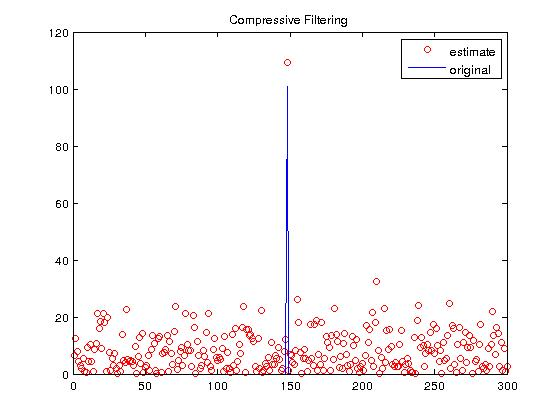
\includegraphics[height = 7.3 cm]{1spike_legend.jpg}
\caption{}
\label{fig:new_basis_25}
\end{figure}

%\inputencoding{latin2}
\bibliography{cswireless2}
%\inputencoding{utf8}

\end{document}